 \section{Simulation}
\label{sec:simulation}

To rigorously evaluate the performance of our proposed joint horizontal-vertical speed optimization algorithm, we consider a multi-rotor UAV deployed for distributed ground nodes data collection missions.

The power consumption of the UAV during horizontal flight is captured by a realistic, empirically validated non-linear function of its forward velocity $v$, expressed as $P_\parallel(v) = c_1 v^3 + c_2 v^2 + c_3 v + P_{mh}$.
Based on empirical flight test configurations from~\cite{Energy-Efficient-POI}, the non-linear coefficients are specified as $c_1 = 0.07$, $c_2 = 0.0391$, and $c_3 = -13.196$, with the baseline hovering power $P_{mh}$ being $390.95$ W .
For vertical flight, we use Eq.~(\ref{equ:v_1}) with $k_1 = 0.8554$, $k_2 = 1.9051$, $c_1 = 0.3177$, and $mg = 63.81\,\mathrm{N}$.
The parameters $k_1$ and $c_1$ are adopted from~\cite{PowerConsumptionModel}, while $k_2$ and $mg$ are calibrated to give a hovering power of approximately $390.8\,\mathrm{W}$, close to the horizontal model's $P_{mh}=390.95\,\mathrm{W}$.
The horizontal and vertical speeds of the UAV are restricted to $V_{\parallel}^{\max} = 20$ m/s and $V_{\perp}^{\max} = 10$ m/s, respectively, while its maximum-range speed-defined as the speed that maximizes aerodynamic efficiency-is determined to be $v_{\mathrm{best}} = 13.99$ m/s by minimizing $P_{\parallel}(v_{\parallel})/v_{\parallel}$.

In our simulation environment, a set of ground nodes (GNs) are deployed along a straight-line, and each $GN_i$ is assigned a random coordinate along the axis.
By default, the total number of GNs, denoted as $N_{GN}$, is set to 20, with spacing between consecutive GNs averaging 60 m.
To emulate realistic deployment heterogeneity, the parameters associated with each GN are not fixed to a single global value: as listed in \textit{Table. \ref{tbl:parameters}}, the parameter of each individual GN is independently and uniformly sampled within its per-GN variation range, so that different GNs within the same mission exhibit heterogeneous communication coverages and data requirements.
On this basis, each controlled experiment varies the default value of one parameter (or two coupled parameters, as in Fig.~(\ref{fig:sim})(f)) at a time, while all the remaining parameters follow the default configuration with the per-GN randomization preserved.

\begin{table}%[]
\caption{Default parameter setting.
The \emph{default value} is the mean used when a parameter is not being scanned; the \emph{per-GN variation range} is the uniform sampling interval for each individual GN.
In each controlled experiment, only the default value of the scanned parameter is varied, while all other parameters are sampled per GN from their variation ranges.}\label{tbl:parameters}
\begin{tabular*}{\tblwidth}{lcc}
\toprule
 Parameter & Default & Variation Range \\ % Table header row
\midrule
 Average\ $PL\ (dB)$ & 85  & [83 86]\\
 Average\ $D_i\ (Mbit)$ & 88 & [72 100]\\
 Nominal\ SINR\ $\Gamma_i$ & 15 & [12 18]\\
 Parameter\ $\mu _{LoS}\ (dB)$& 1.3 & [1 1.6]\\
 Parameter\ $\mu _{NLoS}\ (dB)$& 35 & -\\
 Average distance\ $(m)$& 60 & [30 80]\\
 Altitude\ bounds\ $[h_{\min},h_{\max}]$ (m) & [50, 150] & -\\
 Parameter\ $a$& 45 & [42 47]\\
 Parameter\ $b$& 0.25 & [0.2 0.3]\\
 Average\ number\ of\ $GN$& 20 & -\\
\bottomrule
\end{tabular*}
\end{table}


The air-to-ground wireless links between the flying UAV and the GNs are characterized by the communication model to account for typical urban blocking and shadowing effects.
The probability of establishing an LoS link depends heavily on the elevation angle $\theta$ between the UAV and the target GN, which is mathematically given by Eq.~(\ref{equ:PL}), where the environment-specific parameters are selected as $a = 45$ and $b = 0.25$.
The wireless communication operates at a standard carrier frequency of $f = 2.4 GHz$, with the speed of light defined as $c = 3 \times 10^8$ m/s.
The average excessive path losses for LoS and Non-Line-of-Sight (NLoS) connections are configured as $\mu_{LoS} = 1.3$ dB and $\mu_{NLoS} = 35$ dB, respectively.
A communication link is deemed valid and available for data upload if and only if the total path loss remains below a maximum allowable threshold of $PL = 85$ dB, which defines the continuous geometric coverage boundary shape for each GN.
The data upload adopts a channel bandwidth of $B = 1$ MHz and a per-GN nominal SINR $\Gamma_i$ sampled from $[12, 18]$ (default $15$), which yields a constant achievable rate $\bar{R}_i = B\log_2(1+\Gamma_i)$, about $4$ Mbps at the default. The required collection duration is then $\tau_i = D_i/\bar{R}_i$, which is approximately $22$ s on average under the default data volume $D_i = 88$ Mbit.

Each experimental configuration is repeated over $K = 5$ independent trials.
In every trial, the GN positions and the per-GN parameters are re-sampled uniformly from the variation ranges listed in \textit{Table.\ref{tbl:parameters}}, and the reported energy is the average over the $K$ trials.
The starting altitude is an exogenous mission constraint: the UAV departs and terminates at an altitude of $50$ m in the simulations of Sections~6.1--6.2, and at $100$ m in the real-world case study of Section~6.4.
The flight altitude is confined to $[h_{\min}, h_{\max}]=[50,150]$ m. The lower bound $50$ m matches the take-off/landing altitude, while the upper bound $150$ m is a representative operating ceiling for infrastructure-inspection missions: regulations permit altitudes above the $120$-m open-category limit when the UAV stays in close proximity to a structure (e.g., 14 CFR \S 107.51 allows flying up to 400 ft above a structure's top when within 400 ft of it~\cite{FAA-Part-107}).

% \begin{figure*}%[]
%   \centering
%    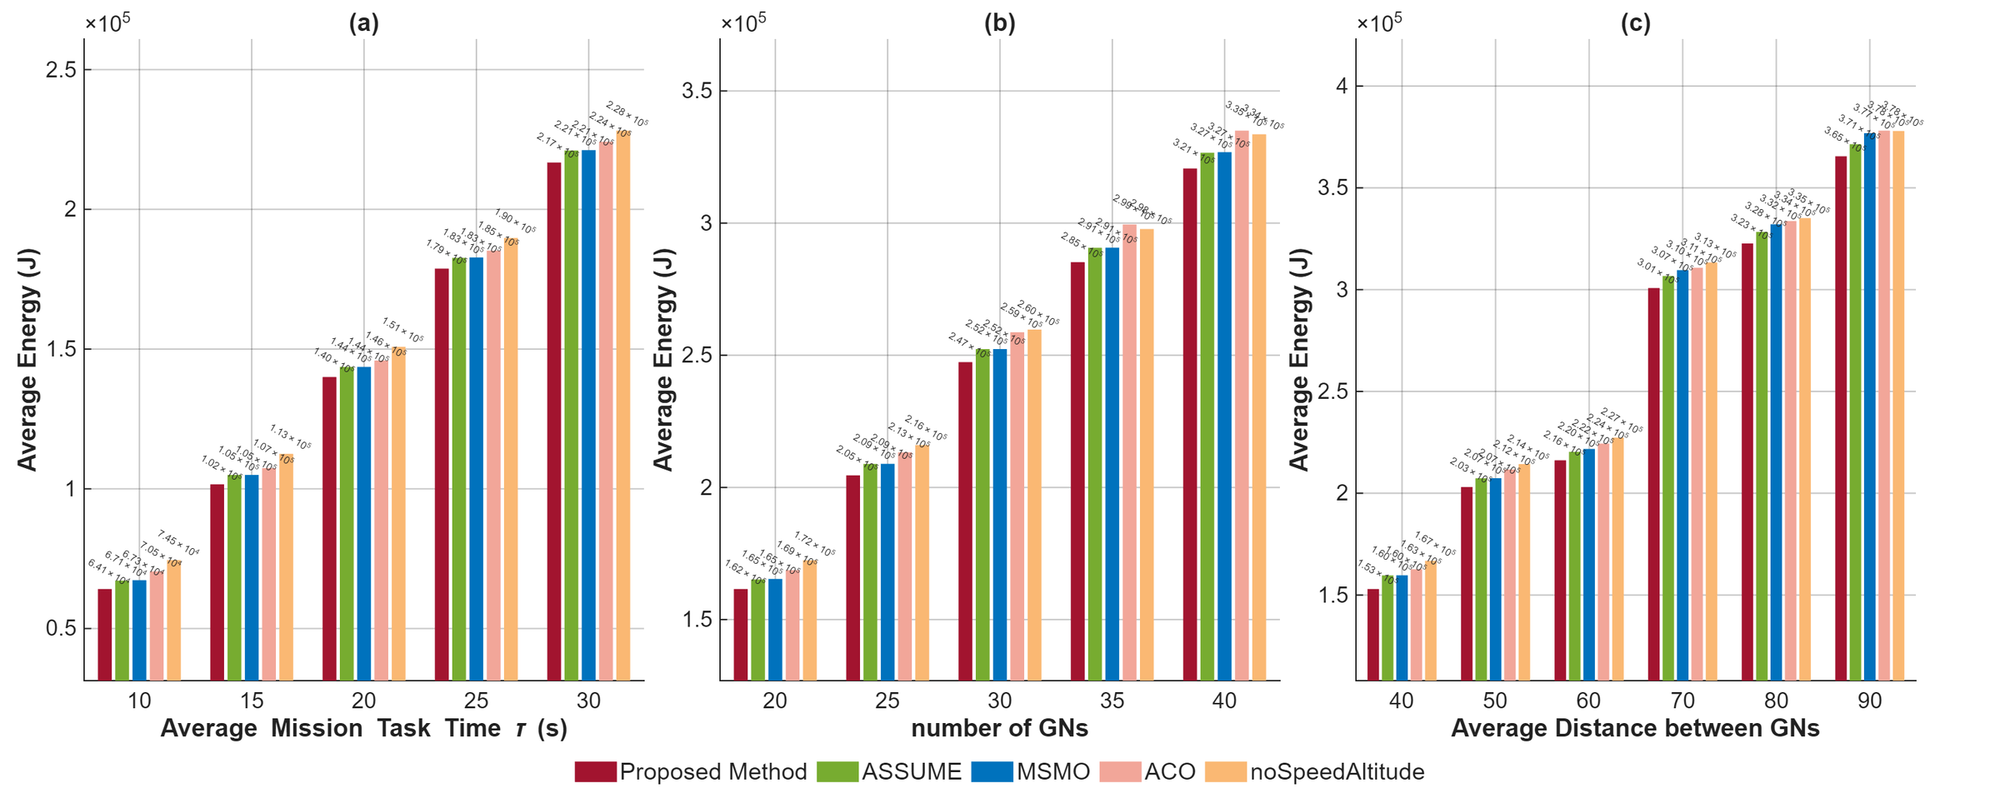
\includegraphics[width = 1\linewidth]{figures/simulation-comparison-alternative.png}
%     \caption{ }\label{fig1}
% \end{figure*}
\subsection{Baseline Algorithms}
We compare our proposed method with following base-line algorithms
\begin{itemize}
    \item \textit{ASSUME~\cite{assume}}: The ASSUME algorithm tackles the joint altitude and speed scheduling problem by discretizing the allowable 3D flight space.
    It quantizes the UAV's flight altitude into a finite set of horizontal segments.
    Within each fixed-altitude layer, it employs the Looking-Before-Crossing (LbC) technique to trace a shortest-path speed schedule across virtual spatial-temporal constraints.
    A dynamic programming (DP) framework is then superimposed to compute the optimal path across these different altitude levels.
    While ASSUME achieves mathematical optimality within its discrete framework, its performance is inherently bottlenecked by the resolution of its pre-defined altitude grid, often suffering from quantization errors that preclude finding the true continuous energy minimum.
    \item \textit{MSMO~\cite{msmo}}: This baseline introduces a speed scheduling that at any given iteration $t$, the UAV's horizontal velocity is dynamically evolved according to the rule: $v^{t}=v^{t-1}+R_{1}(v^{*}-v^{t-1})+R_{2}(1-A)(v_{max}-v_{min})$, where $R_{1}$ and $R_{2}$ are randomized tuning weights.
    The second term explicitly exploits the search space by pulling the speed toward the theoretical optimum $v^{*}$, whereas the third term injects random velocity perturbations to prevent the algorithm from stagnating in local energy minima.
    To handle the 3D environment, this iterative speed evolution is exhaustively repeated across all discrete altitude layers, ultimately outputting the altitude-speed pair that yields the lowest empirical energy cost.
    \item \textit{ACO~\cite{bi-aco}}: This approach decouples the scheduling dimensions, applying a deterministic rule for horizontal speed and a ACO based framework for vertical altitude.
    The horizontal transit speed over any target node $g_{i}$ is strictly dictated by the effective transmission range, calculated as $(f_{i}-\max(s_{i}, f_{i-1})) / \tau_{i}$.
    For the vertical dimension, an Ant Colony Optimization mechanism simulates pheromone deposition and heuristic path generation to navigate the discrete altitude levels.
    \item \textit{noSpeedAltitude}: Serving as a naive, worst-case benchmark, this algorithm entirely eliminates global dynamic optimization.
    Identical to the ACO method, the UAV's horizontal velocity is locked to a rudimentary calculation based on the effective transmission range and required time $\tau_{i}$.
    However, its altitude selection is reduced to a purely greedy mechanism: at each GN transition, the algorithm simply scans all feasible altitudes and forcibly selects the one that physically maximizes the geometric transmission coverage radius.
\end{itemize}
\begin{figure*}%[]
  \centering
   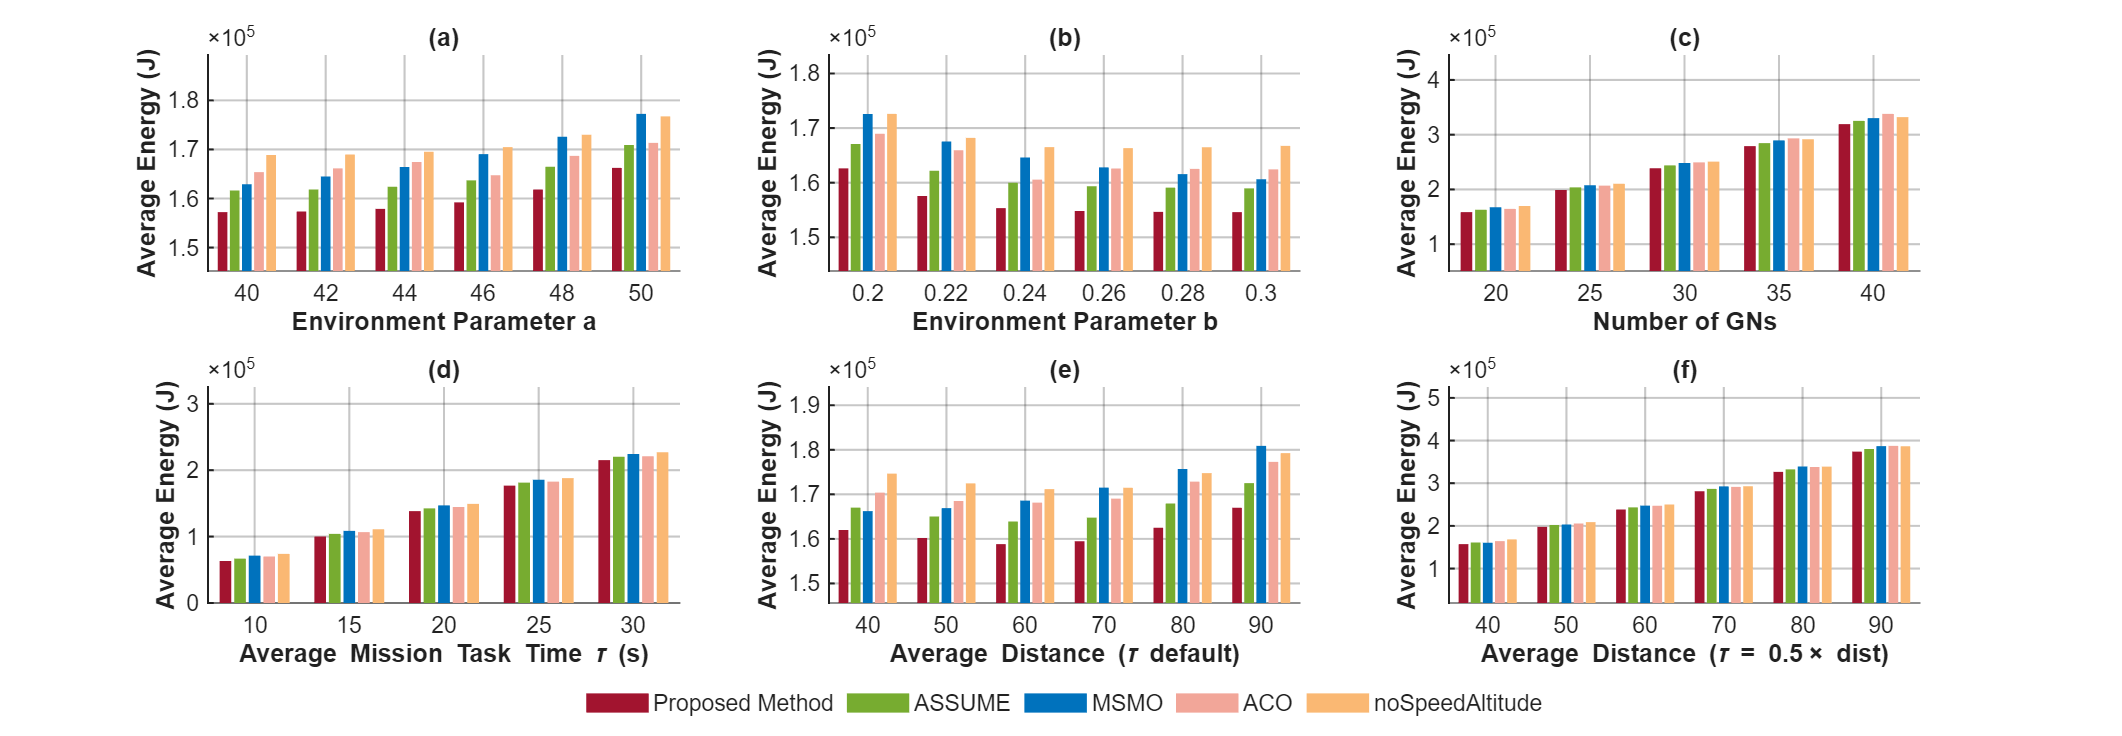
\includegraphics[width = 1.\linewidth]{figures/simulation-comparison.png}
    \caption{The UAV energy consumption of different algorithms.
    In (a), as the environment parameter $a$ --- equivalently, the elevation angle at which the LoS probability reaches $50\%$, given by $a+\ln(a)/b$ --- increases from 40 to 50 (from street canyons to extremely dense high-rise districts), the coverage region of each GN shrinks and the energy consumption of JHVSO, ASSUME, MSMO and noSpeedAltitude increases monotonically, with the increase steepening for $a\ge46$; the margin of JHVSO over MSMO widens from 3.6\% to 6.6\%.
    In (b), as the environment parameter $b$ increases, all methods first decrease in energy consumption and then stabilize once the LoS probability approaches its upper limit, with ACO and noSpeedAltitude showing minor non-monotonic wiggles.
    In (c), the energy consumption for each method increases constantly with more ground nodes added to the mission.
    In (d), all methods have the increase in energy consumption as the average time to complete data collection from one ground node increases.
    (e) and (f) show how the energy consumption of all methods changes as the distance between adjacent ground nodes increases.
    For (e), $\tau$ remains at its default value: the energy of JHVSO, ASSUME, ACO and noSpeedAltitude first decreases slightly (by about 2\%, with the minimum at an average distance of 60 m) and then increases, whereas MSMO rises monotonically, so that the margin of JHVSO over MSMO widens from 2.6\% at 40 m to 8.3\% at 90 m.
    For (f), $\tau$ grows proportionally with the distance, and the energy consumption of all methods increases monotonically.
    JHVSO achieves the lowest energy consumption in all 34 configurations, reducing energy by 1.7\%--5.8\% over the strongest baseline (ASSUME), 1.9\%--12.9\% over MSMO, 2.7\%--10.7\% over ACO, and 3.4\%--16.8\% over the greedy speed--height baseline (noSpeedAltitude).}\label{fig:sim}
\end{figure*}
\subsection{Simulation Results and Comparative Analysis}


Fig.~(\ref{fig:sim}) presents a comprehensive performance evaluation of the proposed \textit{JHVSO} algorithm alongside four baseline methods: ASSUME, MSMO, ACO, and noSpeedAltitude.

To thoroughly investigate the adaptability and robustness of these algorithms under diverse operational environments, we conduct six controlled experiments following the protocol of \textit{Table 1}: in each subfigure, the x-axis denotes the varied default value of the corresponding parameter, while the per-GN randomization within the variation ranges of \textit{Table 1} is preserved.
Each configuration is evaluated on three independent random instances, and the reported value is the average over the three instances.
To isolate the effect of the swept parameter from instance-to-instance fluctuations, the same random instances are reused across all sweep points of an experiment (common random numbers) so that only the swept parameter differs between neighboring points of a curve.

In Fig.~(\ref{fig:sim})(a), we evaluate the energy consumption as the environment parameter $a$ increases from 40 to 50.
Here the elevation angle $\theta=\arctan(h/d)$ measures how steeply the UAV looks down at a GN: $\theta=90^{\circ}$ corresponds to hovering directly overhead, while a small $\theta$ corresponds to a grazing link that has to pass through the surrounding buildings.
Buildings therefore block the link at low elevations, so that the LoS probability follows the S-curve of Eq.~(\ref{equ:PL}) and reaches $50\%$ at $\theta_{50}=a+\ln(a)/b$; at the nominal value $b=0.25$, $\theta_{50}$ rises from about $55^{\circ}$ to about $66^{\circ}$ as $a$ increases from 40 to 50, which means that at a flight height of 100 m the horizontal distance at which a link is equally likely to be LoS or NLoS decreases from about 70 m to about 45 m (the actual coverage boundary lies somewhat above $\theta_{50}$ because the NLoS excess loss is large).
A larger $a$ therefore corresponds to a harsher propagation environment, in which the coverage region of each GN is smaller and the feasible collection windows are tighter.
As shown in the figure, the energy consumption of JHVSO, ASSUME, MSMO and noSpeedAltitude increases monotonically with $a$, while ACO exhibits a minor fluctuation at $a=46$ due to its randomized search.
For JHVSO the increase is gradual below $a=44$ ($+0.1\%$ and $+0.4\%$ per 2-unit step) and steepens for $a\ge46$ ($+0.8\%$, $+1.7\%$ and $+2.7\%$ per step), reflecting the accelerating shrinkage of the coverage regions.
The relative ranking of the five methods is stable across all settings, with the proposed JHVSO algorithm consistently achieving the lowest energy consumption.
Quantitatively, JHVSO reduces energy consumption by 2.8\%--2.9\% over ASSUME (the strongest competing baseline), by 3.6\%--6.7\% over MSMO, by 3.1\%--6.0\% over ACO, and by 6.3\%--7.4\% over the greedy noSpeedAltitude baseline; the largest saving occurs at $a=40$, where JHVSO consumes $1.57\times10^{5}$ J against $1.69\times10^{5}$ J of noSpeedAltitude, i.e., a 7.4\% energy saving.
Notably, the margin over MSMO grows from 3.6\% at $a=40$ to 6.6\% at $a=50$, indicating that the advantage of joint speed-altitude optimization becomes more pronounced as the environment deteriorates.

In Fig.~(\ref{fig:sim})(b), we examine the effect of the environmental parameter $b$, which controls the sensitivity of the LoS probability to the elevation angle in Eq.~(\ref{equ:PL}).
An increase in $b$  raises the LoS probability at a given elevation angle and thereby effectively expands the communication coverage, providing the UAV with larger feasible windows for data collection.
Consequently, the energy consumption of all methods first decreases as $b$  grows: for JHVSO the drop is 3.1\% at the first step ($b=0.22$) and 1.4\% at $b=0.24$.
Beyond this point, however, the $LoS$ probability gradually saturates---as the sigmoid in Eq.~(\ref{equ:PL}) approaches its upper limit---so that the coverage barely expands any further and the energy consumption of JHVSO and ASSUME remains virtually flat up to $b=0.3$.
The small non-monotonic wiggles of ACO and noSpeedAltitude (e.g., noSpeedAltitude turns upward after $b=0.26$) stem from their altitude-selection heuristics, which respond to the enlarged coverage by shifting to higher cruising altitudes and thus incurring extra climb and descent costs.
Throughout this sweep, JHVSO maintains the lowest energy footprint, reducing consumption by 2.8\%--3.0\% over ASSUME, by 3.9\%--6.3\% over MSMO, and by 6.1\%--7.9\% over noSpeedAltitude; the peak reduction of 7.9\% is observed at $b=0.3$ ($1.55\times10^{5}$ J versus $1.67\times10^{5}$ J).

As depicted in Fig.~(\ref{fig:sim})(c) and Fig.~(\ref{fig:sim})(d), the energy consumption of all evaluated methods scales upward under increasing mission workloads.
Specifically, Fig.~(\ref{fig:sim})(c) shows a monotonic rise in total energy expenditure as more GNs are integrated into the flight mission.
Across all deployment scales from 20 to 40 GNs, JHVSO reduces energy consumption by 1.8\%--2.7\% over ASSUME, by 3.4\%--5.6\% over MSMO, by 3.8\%--5.8\% over ACO, and by 4.0\%--7.1\% over noSpeedAltitude, with the largest gain (7.1\%) achieved at the 20-GN scale ($1.59\times10^{5}$ J versus $1.70\times10^{5}$ J).
Similarly, Fig.~(\ref{fig:sim})(d) indicates that extending the average minimum required data collection time ($\tau$) per GN intrinsically demands prolonged flight or hovering durations, thereby consistently elevating the overall energy consumption across all algorithms.
This setting yields the most pronounced relative advantage of JHVSO among all experiments: at $\tau=10$ s the energy reduction reaches 5.8\% over ASSUME, 12.9\% over MSMO, 10.7\% over ACO, and 16.8\% over noSpeedAltitude ($6.32\times10^{4}$ J versus $6.69\times10^{4}$ J, $7.14\times10^{4}$ J, $7.00\times10^{4}$ J, and $7.39\times10^{4}$ J, respectively). As $\tau$ grows to 30 s, the collection time progressively dominates the total mission energy, so the relative margins narrow to 2.3\% (ASSUME), 4.2\% (MSMO), 2.7\% (ACO), and 5.5\% (noSpeedAltitude), yet JHVSO remains the most energy-efficient method at every data point.

Fig.~(\ref{fig:sim})(e) and Fig.~(\ref{fig:sim})(f) explore the algorithmic performance as the average distance between GNs increases.
In Fig.~(\ref{fig:sim})(e), the required task time $\tau$ is kept constant.
As the inter-node distance grows, the UAV is compelled to increase its average transit speed, which better aligns with the optimal aerodynamic cruising speed.
For small spacings, the coverage regions of adjacent GNs still overlap, so that the collection segment itself covers the entire transition and the energy consumption of JHVSO, ASSUME, ACO and noSpeedAltitude decreases slightly (by about 2\%) and reaches its minimum at an average distance of 60 m.
Beyond 60 m, the coverage regions separate, so that the UAV has to cruise outside the coverage in the gaps between nodes; this additional distance outweighs the speed benefit and the energy consumption of these four methods rises again.
MSMO, in contrast, exhibits a monotonic performance degradation over the entire range, indicating a higher susceptibility to suboptimal scheduling within extended gap segments.
Consequently, JHVSO's advantage over MSMO widens from 2.6\% at 40 m to 8.3\% at 90 m, while its margin over ASSUME remains at about 3.1\%--3.4\% and its margin over noSpeedAltitude at about 7.3\%--7.8\% throughout the sweep.
In Fig.~(\ref{fig:sim})(f), $\tau$ scales proportionally with the inter-node distance (fixed ratio of 0.5).
Under this coupled constraint, the extended spatial traversal strictly mandates a correspondingly longer mission duration, resulting in a predictable and consistent increase in energy consumption across all methods.
Even so, JHVSO reduces energy consumption by 1.7\%--2.4\% over ASSUME, by 1.9\%--4.0\% over MSMO, and by 3.4\%--7.0\% over noSpeedAltitude, again peaking at 7.0\% for the 40 m spacing ($1.57\times10^{5}$ J versus $1.68\times10^{5}$ J).

In summary, throughout all 34 experimental configurations in Fig.~(\ref{fig:sim}), the proposed JHVSO method consistently maintains the lowest energy consumption footprint, reducing energy consumption by up to 16.8\% over the greedy speed-height baseline and by up to 5.8\% over the strongest competing baseline (ASSUME).

\subsection{Discretization Sensitivity and Computational Cost}

The global optimality guarantee of the proposed \textit{ORE} algorithm holds over the discretized state space, i.e., over the finite set of candidate states sampled within the communication region of each GN. Concretely, the continuous communication region of each GN is first rasterized onto a fine grid in the $(d,h)$ plane with a resolution of $1$ m, which yields the full set of candidate state points located inside the coverage region. When a GN contains more candidate points than a prescribed cap $M$, the points are uniformly subsampled in raster order---keeping every $s$-th point with $s=\lfloor N_c/M \rfloor$, where $N_c$ is the number of candidate points of that GN---so that approximately $M$ states remain; GNs whose coverage contains no more than $M$ candidate points keep all of them. As a result, the actual number of sampled states of each GN fluctuates around $M$ depending on its coverage area (on average approximately $2357$ and $5791$ states for $M=2000$ and $M=4000$, respectively). To assess the impact of this sampling resolution, we evaluate the algorithm under different caps $M \in \{250, 500, 1000, 2000, 4000\}$.

\begin{table*}[]
\caption{Total energy and relative improvement of each of the five experiments under different state sampling caps $M$. The relative improvement columns report the percentage reduction in energy when the cap is refined to the next resolution, e.g., $(E_{250}-E_{500})/E_{250}$. The energy decreases monotonically and converges as $M$ increases, with only a small difference across the resolutions.}\label{tbl:sensitivity}
\begin{tabular*}{\textwidth}{l ccccc cccc}
\toprule
 & \multicolumn{5}{c}{Total energy (J)} & \multicolumn{4}{c}{Relative improvement (\%)} \\
\cmidrule(lr){2-6} \cmidrule(lr){7-10}
 Exp & $M=250$ & $M=500$ & $M=1000$ & $M=2000$ & $M=4000$ & $250\!\to\!500$ & $500\!\to\!1000$ & $1000\!\to\!2000$ & $2000\!\to\!4000$ \\
\midrule
 Exp.\ 1 & 153946 & 153558 & 153370 & 153315 & 153178 & 0.2520 & 0.1224 & 0.0361 & 0.0895 \\
 Exp.\ 2 & 162798 & 162207 & 162005 & 161858 & 161742 & 0.3630 & 0.1243 & 0.0907 & 0.0717 \\
 Exp.\ 3 & 151038 & 150486 & 150338 & 150171 & 150078 & 0.3657 & 0.0982 & 0.1107 & 0.0625 \\
 Exp.\ 4 & 153148 & 152940 & 152693 & 152600 & 152535 & 0.1363 & 0.1612 & 0.0609 & 0.0428 \\
 Exp.\ 5 & 155466 & 155100 & 155092 & 155001 & 154873 & 0.2359 & 0.0052 & 0.0584 & 0.0824 \\
\midrule
 Mean & 155279 & 154858 & 154700 & 154589 & 154481 & 0.2706 & 0.1023 & 0.0714 & 0.0698 \\
\bottomrule
\end{tabular*}
\end{table*}

\begin{figure}%[]
  \centering
   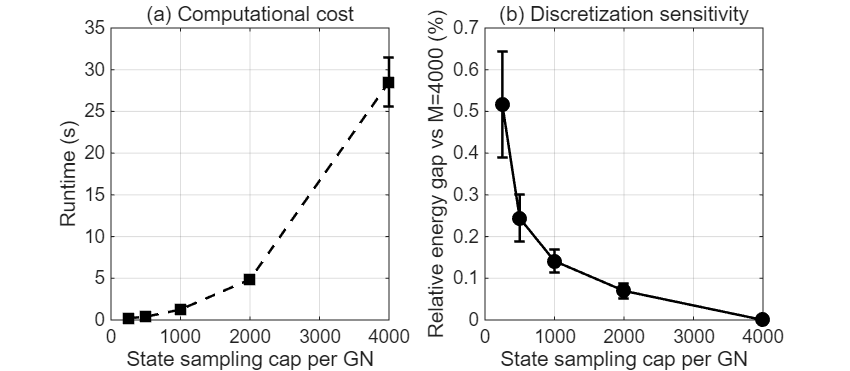
\includegraphics[width = 1\linewidth]{figures/discretization-sensitivity.png}
    \caption{Discretization sensitivity and computational cost. (a) Running time and (b) the relative optimality gap with respect to the finest resolution $M=4000$, versus the state sampling cap $M$. Each point is averaged over five random scenarios, with error bars denoting the standard deviation.}\label{fig:sensitivity}
\end{figure}

As shown in Table~\ref{tbl:sensitivity}, the total energy of every experiment decreases monotonically and converges as $M$ increases. On average, refining $M$ from $1000$ to $4000$ reduces the total energy by only $0.14\%$, and the improvement shrinks as the resolution doubles, indicating approximately first-order convergence (Fig.~(\ref{fig:sensitivity})(b)). At the operating resolution $M=2000$, the optimal energy is within $0.07\%$ of that obtained at $M=4000$; this residual gap reflects the discretization error of the state space and is negligible in practice, confirming that the discretized optimum has essentially converged to the continuous optimum. Meanwhile, as shown in Fig.~(\ref{fig:sensitivity})(a), the running time grows with $M$, averaging $4.86$ s at the operating resolution $M=2000$. Overall, a sampling cap in the range $M \in [1000, 2000]$ strikes a good balance between energy optimality and computational cost. Notably, even the coarsest resolution $M=250$ is only about $0.5\%$ above the finest $M=4000$, confirming that the discretization resolution has only a marginal impact on the optimal energy and mainly affects the computational cost.

\subsection{Real World Scenario Case Study}

\begin{figure}%[]
  \centering
   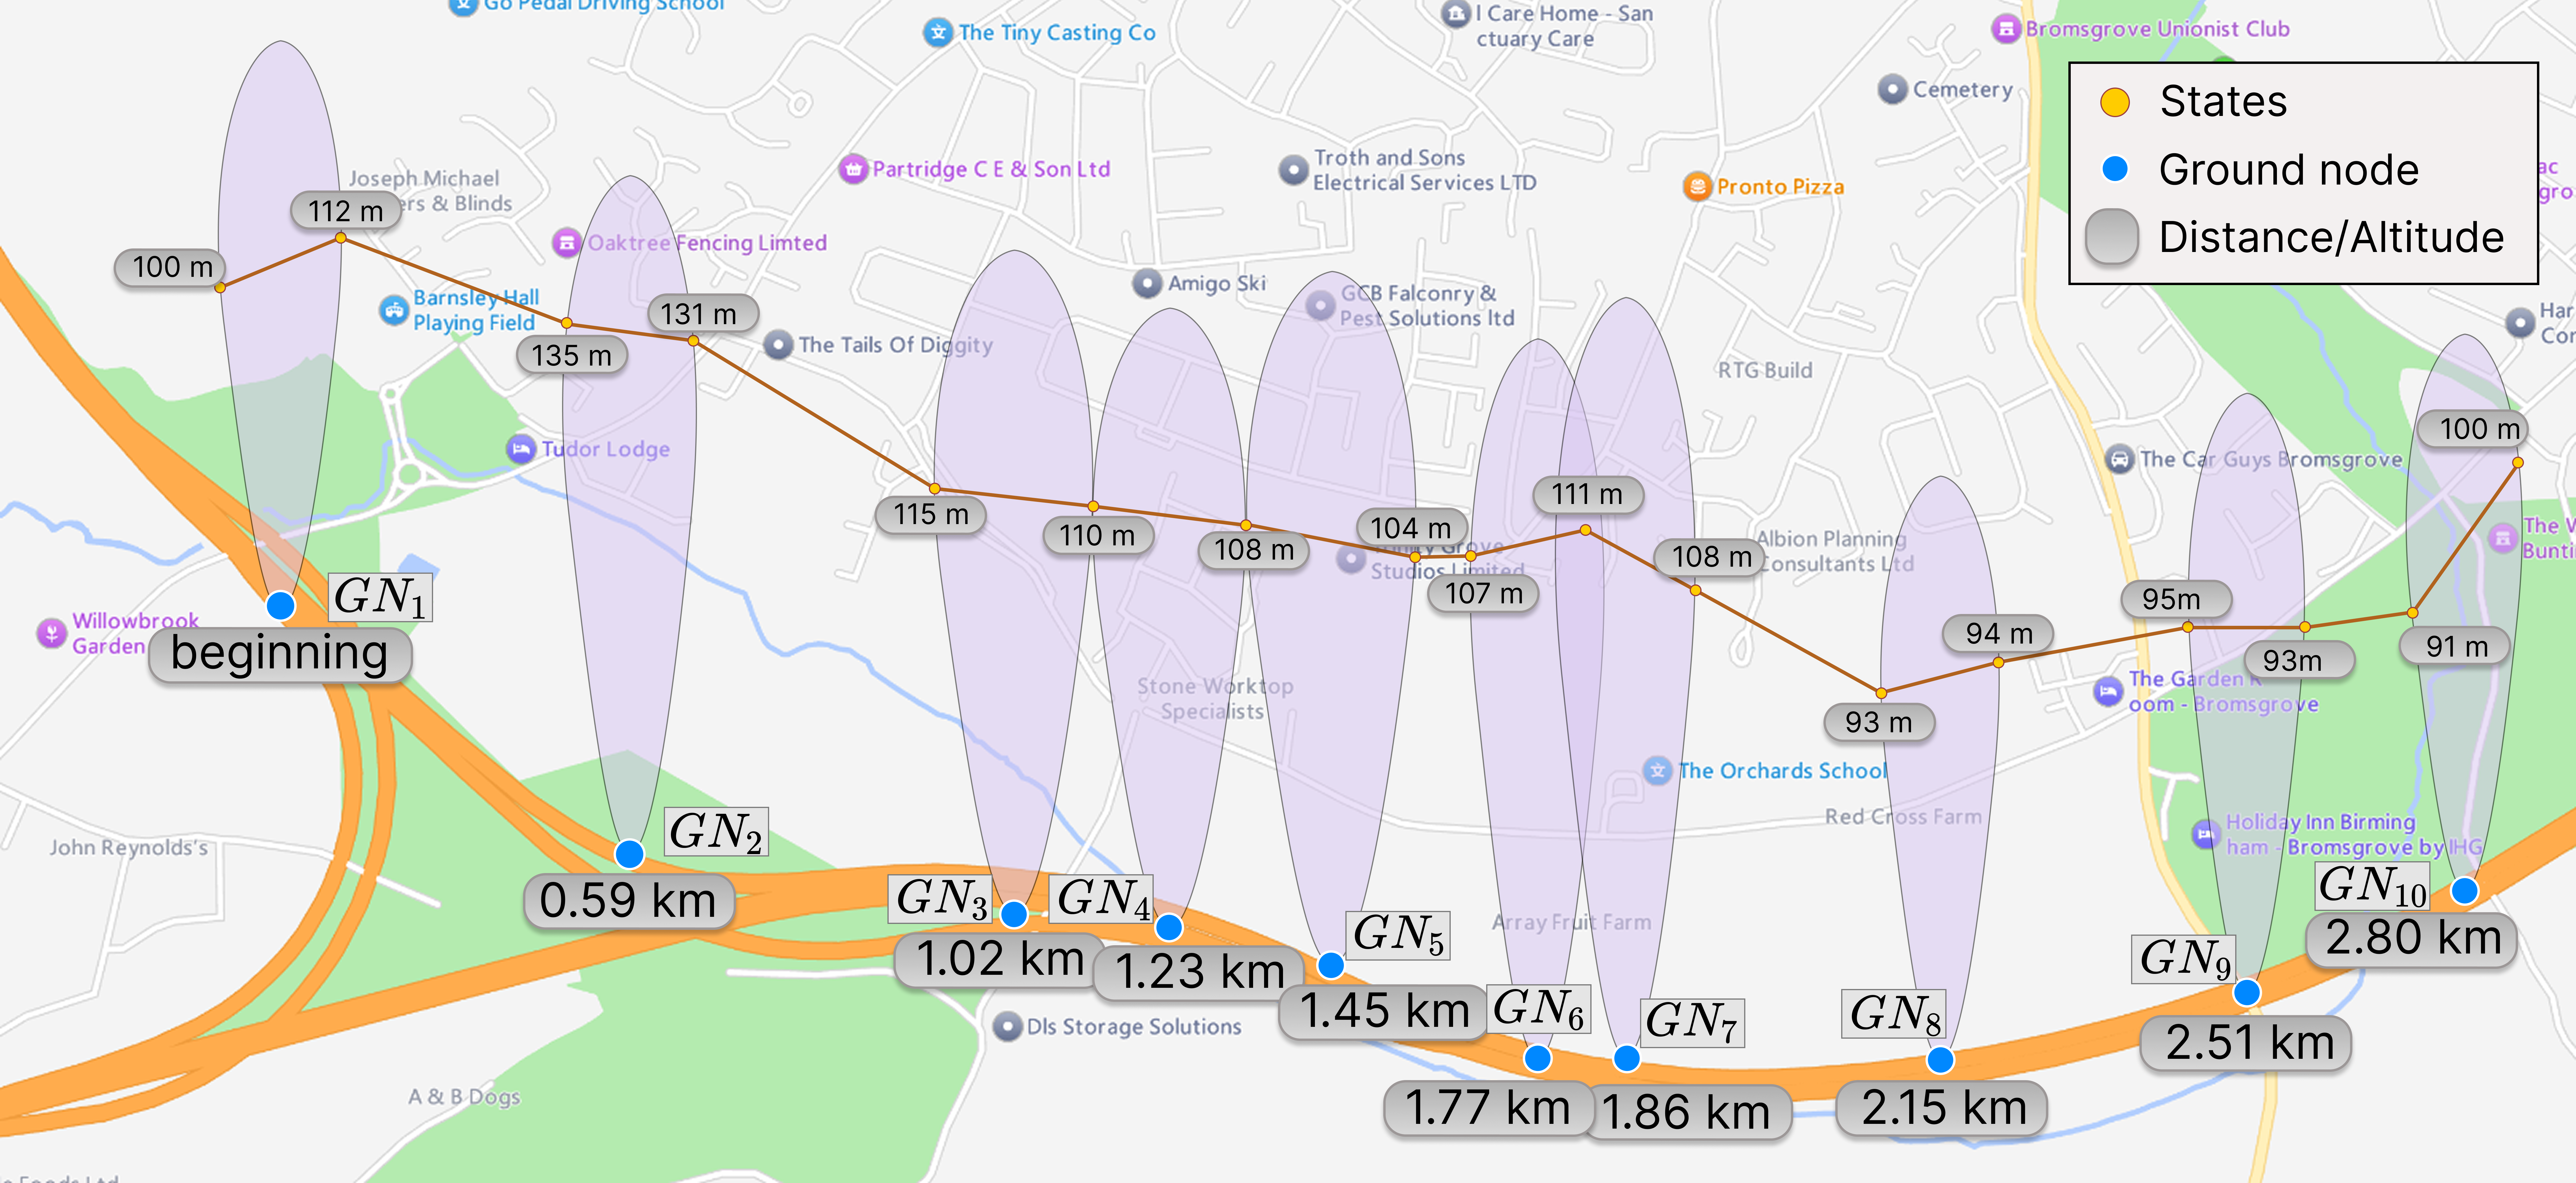
\includegraphics[width = 1\linewidth]{figures/real-world-scenario.png}
    \caption{The traffic CCTVs at M5, Bromsgrove, England, United Kingdom~\cite{UKLiveCamera}}\label{fig:real_scenario}
\end{figure}

\begin{table}%[]
\caption{Per-segment speed schedule of the \textit{JHVSO}-planned trajectory in the real-world scenario.}\label{tbl2}
\begin{tabular*}{\tblwidth}{lcccr}
\toprule
 Segment & Type & $v_\parallel (m/s)$ & $v_\perp$ & Duration (s) \\ % Table header row
\midrule
$GN_1$ & Task  & 7.00  & 0.57  & 21.00\\
$GN_2$ & Gap   & 13.94 & 0.80  & 28.76\\
$GN_2$ & Task  & 12.17 & -0.17 & 18.00\\
$GN_3$ & Gap   & 13.94 & -1.16 & 14.70\\
$GN_3$ & Task  & 11.40 & -0.25 & 20.00\\
$GN_4$ & Task(direct)  & 8.86  & -0.09 & 22.00\\
$GN_5$ & Task(direct)  & 12.89 & -0.21 & 19.00\\
$GN_6$ & Gap   & 13.96 & 0.38  & 7.81 \\
$GN_6$ & Task  & 8.94  & 0.24  & 17.00 \\
$GN_7$ & Task(direct)  & 9.17  & -0.25 & 12.00 \\
$GN_8$ & Gap   & 13.92 & -1.63 & 9.20 \\
$GN_8$ & Task  & 7.09  & 0.05  & 22.00 \\
$GN_9$ & Gap   & 13.96 & 0.07  & 14.54 \\
$GN_9$ & Task  & 7.18  & -0.09 & 22.00 \\
$GN_{10}$ & Gap   & 13.96 & -0.20 & 10.10 \\
$GN_{10}$ & Task  & 6.95  & 0.47 & 19.00 \\
\bottomrule
\end{tabular*}
\end{table}

We conduct a simulation using the real-world dataset, contains 10 public traffic CCTV cameras places at high way in Deciduous Broadleaf, England ,United Kingdom.
We assume that the UAV is deployed to collect data from these cameras.
Then by using our proposed \textit{JHVSO} algorithm, we scheduled the speed and altitude use for the mission , the UAV is constrained to start the mission at an altitude of 100 m at the first GN (i.e., $h_{0} = 100m$ in \textit{Definition. \ref{def:JHVSO}}), and the trajectory terminates at an altitude of 100 m within the communication region of the last GN.

\textit{Table. \ref{tbl2}} details the speed schedule of the planned trajectory on a per-segment basis.
In the Gap segments, the UAV cruises at horizontal speeds of $13.92-13.96 m/s$ with small vertical components bounded within $\pm 1.63 m/s$, and the segment durations range from $7.81 s$ to $28.76 s$, varying with the spacing between the coverage regions of adjacent GNs.
In the Task segments, the UAV slows down to $6.95-12.89 m/s$, and the duration of each Task segment equals the required collection time of the corresponding GN.
Notably, the transitions toward $GN_5$ and $GN_7$ contain no Gap segment, as the UAV has not yet left the communication coverage of the next GN upon finishing the previous collection task.
Overall, the mission is completed in $278 s$, of which $85.1 s\ (\approx30 \%)$ is spent on inter-node cruising.



%%%%%%%%%%%%%%%%%%%%%%%%%%%%%%%%%%%%%%%%%%%%%%%%%%%%%%%%%%%%%%%%%%%%%%%%%%%%%%%%%%
%%%%%%%%%%%%%%%%%%%%%%%%%%%%%%%%%%%%%%%%%%%%%%%%%%%%%%%%%%%%%%%%%%%%%%%%%%%%%%%%%%
